\documentclass[11pt]{article}
\usepackage[a5paper, left=5mm, right=5mm, top=5mm, bottom=5mm]{geometry}
\usepackage{cmap} % улучшенный поиск русских слов в pdf
\usepackage[T2A]{fontenc}
\usepackage[utf8]{inputenc}
\usepackage{multicol}
\usepackage[english, russian] {babel}
\usepackage{amsfonts,ams symb}
\usepackage{graphicx} 
\graphicspath{ {images/} }
\usepackage{float} 
\usepackage{makecell}
\usepackage{footnote}
\usepackage{footmisc}
\renewcommand{\thefootnote}{\textnormal{*)}}
\usepackage{caption}
\usepackage{rotating}
\captionsetup[figure]{labelsep=none}
\begin{document}
\begin{multicols}{2}
    \small
    Величину
    \[\lambda = \frac{1}{2h} = \frac{1}{2 \cdot \left|q \alpha - p\right|}\]
    назовем коэффициентом выгодности. Его смысл очень прост: коэффициент выгодности показывает, во сколько раз фактическая абсолютная погрешность меньше максимально возможной. Чем больше 2, тем выгоднее приближение. Очевидно,
    \[1\leq \lambda < \infty\]
    \[\lambda h = \frac{1}{2}\]

    Не следует думать, что более мел- кие доли всегда дают более точное приближение! Может случиться, что при нанесении на числовую ось вось- мых долей число а занимает менее выгодное положение, чем при на- несении седьмых. Сделаем опыт с числом л, аппроксимируя его разны- ми долями - от первых до десятых. Вычисления опущены, читатель мо- жет воспроизвести их сам.
    \begin{table}[H]
    \tiny
    \begin{tabular}{c|c|c|c|c|c}
        \hline
        q & \rotatebox{90}{\makecell{приближенное \\ значение $\pi$ \vspace{5pt}}} & \makecell{верхняя \\ граница \\ абсолютной \\ пргрешности}
        & $\Delta$ & h & $\lambda$ \\
        \hline
        1 & $\frac{3}{1}$ & $\frac{1}{2}=0,5000$ & 0,1416 & 0,1416 & 3,5 \\
        2 & $\frac{6}{2}$ & $\frac{1}{4}=0,2500$ & 0,1416 & 0,2832 & 1,8 \\
        \hline
    \end{tabular}
    \small
    \end{table}
    
    Эта таблица показывает, что для аппроксимации и седьмые доли резко выгоднее ближайших соседних долей. 
    Фактическая погрешность в 56 раз меньше, чем можно думать, судя по размеру долей
    \footnote{Вычисление дает $\lambda=\frac{1}{2 \cdot 0,0089}=56,2$. 
    Чтобы правильно получить цифры десятых, надо взять и с пятью цифрами после запятой}
    
    На рисунке 2 показано располо- жение числа $\pi$ на числовой оси. Слу- чайно (а впрочем, случайно ли?) $\pi$ оказывается очень близко к 3$\frac{1}{7}$. Если бы нам заранее предписали аппрок- симировать так, чтобы абсолютная \\
    \begin{figure}[H]
        % \centering
        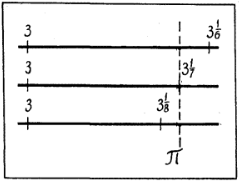
\includegraphics[width=\linewidth]{image2}
        \label{fig:image2} % создание ссылки для последующих обращений
        \caption{}
    \end{figure}
    погрешность не превысила 0,0013, ка- кие доли выбрали бы? Мы записали бы условие $\frac{1}{2q}\geq 0,1300$, откуда $q\geq 4385$,
    а Архимед достиг той же точности, взяв гораздо меньший знаменатель.
    
    Теперь вы убедились, читатель, что Архимед выбрал седьмые доли не случайно?
    
    Через много веков голландский ма тематик Адриан Меций дал прибли- женное значение
    \[\pi \approx \frac{355}{113}\]
    Число Меция обладает теми же уди вительными свойствами, что и число Архимеда: знаменатель 113 гораздо 
\end{multicols}
\end{document}
